\documentclass[border=4pt]{standalone}
% Shared typography and colours for the standalone figures.
\usepackage{unicode-math}
\setmainfont{TeX Gyre Termes}
\setmathfont{TeX Gyre Termes Math}
\usepackage{tikz}
\usetikzlibrary{arrows.meta,positioning,calc,decorations.pathreplacing}
\usepackage{pgfplots}
\pgfplotsset{compat=1.18}
\definecolor{elemA}{HTML}{1F5FA8}
\definecolor{elemB}{HTML}{B8461B}
\definecolor{elemC}{HTML}{2E7D32}
\definecolor{elemD}{HTML}{6A4C93}
\definecolor{frameline}{HTML}{555555}

\begin{document}
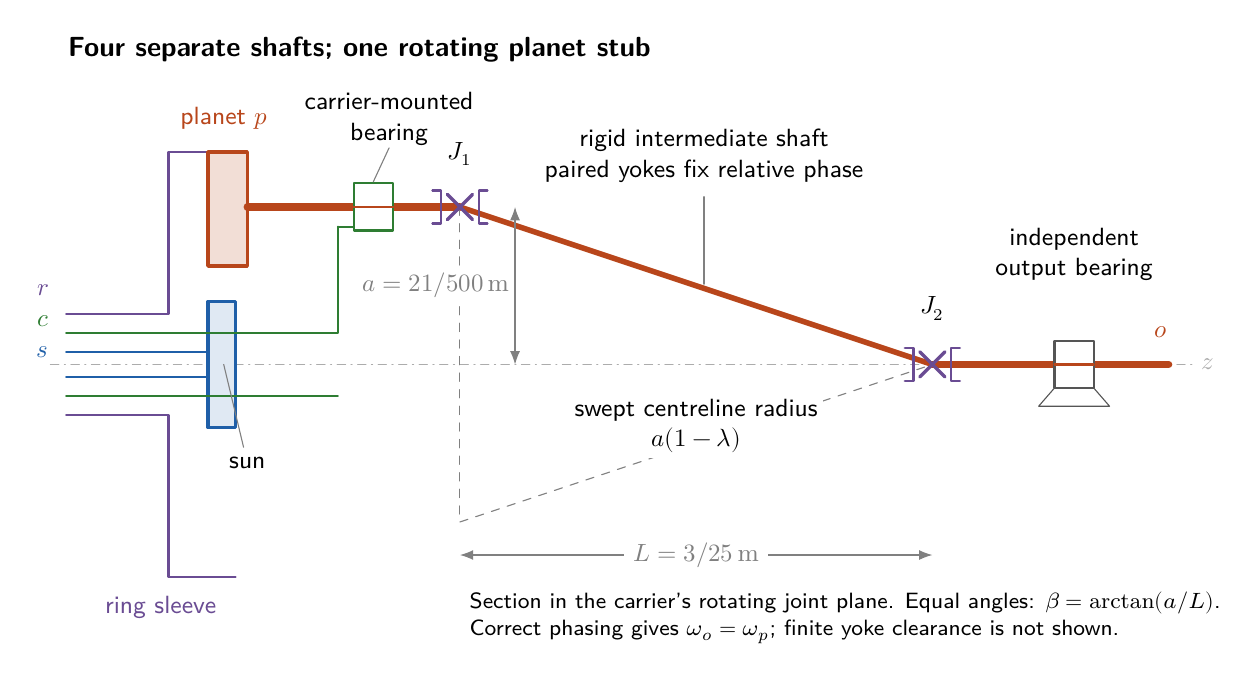
\begin{tikzpicture}[font=\sffamily\small,>=Latex,line cap=round,line join=round]
\draw[gray!65,dash dot] (-1.2,0)--(13.3,0) node[right] {$z$};
\node[anchor=west,font=\sffamily\bfseries] at (-1.1,4) {Four separate shafts; one rotating planet stub};
% Gear members at the left: axial section, with separate sleeves.
\fill[elemA!14] (.8,-.8) rectangle (1.15,.8);
\draw[elemA,very thick] (.8,-.8) rectangle (1.15,.8);
\draw[elemA,thick] (-1,.16)--(.8,.16) (-1,-.16)--(.8,-.16);
\draw[elemC,thick] (-1,.40)--(2.45,.40)--(2.45,1.75)
 (-1,-.40)--(2.45,-.40);
\draw[elemD,thick] (-1,.64)--(.3,.64)--(.3,2.7)--(1.15,2.7)
 (-1,-.64)--(.3,-.64)--(.3,-2.7)--(1.15,-2.7);
\fill[elemB!18] (.8,1.25) rectangle (1.3,2.7);
\draw[elemB,very thick] (.8,1.25) rectangle (1.3,2.7);
\node[elemA,anchor=east] at (-1.1,.16) {$s$};
\node[elemC,anchor=east] at (-1.1,.55) {$c$};
\node[elemD,anchor=east] at (-1.1,.94) {$r$};
\node[align=center] (sunlabel) at (1.3,-1.25) {sun};
\draw[gray] (sunlabel)--(1,.0);
\node[elemD,align=center] at (.2,-3.08) {ring sleeve};
\node[elemB,align=center] at (1,3.13) {planet $p$};
% Stub, support bearing, and first universal joint.
\draw[elemB,line width=2.7pt] (1.3,2)--(4,2);
\filldraw[fill=white,draw=elemC,thick] (2.65,1.7) rectangle (3.15,2.3);
\draw[elemB,thick] (2.65,2)--(3.15,2);
\draw[elemC,thick] (2.45,1.75)--(2.65,1.75);
\node[align=center] at (3.1,3.12) {carrier-mounted\\ bearing};
\draw[gray] (3.1,2.75)--(2.9,2.32);
% Equal-angle parallel-offset lead-out and its swept centreline.
\draw[gray,dashed] (4,-2)--(10,0);
\draw[gray,dashed] (4,2)--(4,-2);
\draw[elemB,line width=2pt] (4,2)--(10,0);
\draw[elemB,line width=2.7pt] (10,0)--(13,0);
\foreach \x/\y in {4/2,10/0}{
 \draw[elemD,line width=1.2pt] (\x-.16,\y-.16)--(\x+.16,\y+.16)
 (\x-.16,\y+.16)--(\x+.16,\y-.16);
 \draw[elemD,thick] (\x-.35,\y-.21)--(\x-.24,\y-.21)--(\x-.24,\y+.21)--(\x-.35,\y+.21);
 \draw[elemD,thick] (\x+.35,\y-.21)--(\x+.24,\y-.21)--(\x+.24,\y+.21)--(\x+.35,\y+.21);
}
\node[above] at (4,2.4) {$J_1$};
\node[above] at (10,.44) {$J_2$};
\node[align=center] at (7.1,2.65) {rigid intermediate shaft\\paired yokes fix relative phase};
\draw[gray] (7.1,2.13)--(7.1,1.02);
\filldraw[fill=white,draw=frameline,thick] (11.55,-.30) rectangle (12.05,.30);
\draw[elemB,thick] (11.55,0)--(12.05,0);
\draw[frameline] (11.55,-.30)--(11.35,-.53)--(12.25,-.53)--(12.05,-.30);
\node[align=center] at (11.8,1.4) {independent\\output bearing};
\node[elemB,above] at (12.9,.22) {$o$};
\draw[<->,gray] (4,-2.42)--(10,-2.42) node[midway,fill=white] {$L=3/25\,\mathrm m$};
\draw[<->,gray] (4.7,0)--(4.7,2) node[midway,left,fill=white,inner sep=2pt] {$a=21/500\,\mathrm m$};
\node[align=center,fill=white,inner sep=2pt] at (7,-.78) {swept centreline radius\\$a(1-\lambda)$};
\node[align=left,anchor=west,font=\sffamily\footnotesize] at (4,-3.22)
 {Section in the carrier's rotating joint plane. Equal angles: $\beta=\arctan(a/L)$.\\
 Correct phasing gives $\omega_o=\omega_p$; finite yoke clearance is not shown.};
\end{tikzpicture}
\end{document}
